\documentclass[tikz,border=2pt,11pt]{standalone}
\usetikzlibrary{arrows.meta}
\usetikzlibrary{calc}
\usetikzlibrary{positioning}
\usepackage{amsmath}
\usepackage{amssymb}
\usepackage{xcolor}
\usepackage{tikz}
\DeclareMathOperator{\Ric}{Ric}
\DeclareMathOperator{\Hess}{Hess}
\DeclareMathOperator{\tr}{tr}
\DeclareMathOperator{\sym}{sym}
\DeclareMathOperator{\supp}{supp}
\DeclareMathOperator{\divg}{div}
\DeclareMathOperator{\id}{id}
\DeclareMathOperator{\rank}{rank}
\DeclareMathOperator{\Lip}{Lip}
\DeclareMathOperator{\Vol}{Vol}
\DeclareMathOperator{\Area}{Area}
\DeclareMathOperator{\dist}{dist}
\DeclareMathOperator{\sgn}{sgn}
\newcommand{\R}{\mathbb R}
\begin{document}
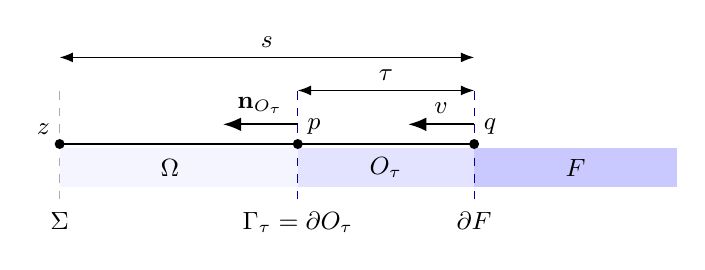
\begin{tikzpicture}[x=1.12cm,y=1cm,>=Latex,font=\small]
 \fill[blue!4] (0,-.55) rectangle (7,-.05);
 \fill[blue!11] (2.7,-.55) rectangle (7,-.05);
 \fill[blue!21] (4.7,-.55) rectangle (7,-.05);
 \draw[gray!65,dashed] (0,-.7)--(0,.7);
 \draw[blue!60!black,dashed] (2.7,-.7)--(2.7,.7);
 \draw[blue!60!black,dashed] (4.7,-.7)--(4.7,.7);
 \draw[thick] (0,0)--(4.7,0);
 \fill (0,0) circle (1.8pt);
 \fill (2.7,0) circle (1.8pt);
 \fill (4.7,0) circle (1.8pt);
 \node[above left] at (0,0) {$z$};
 \node[above right] at (2.7,0) {$p$};
 \node[above right] at (4.7,0) {$q$};
 \node[below] at (0,-.74) {$\Sigma$};
 \node[below] at (2.7,-.74) {$\Gamma_\tau=\partial O_\tau$};
 \node[below] at (4.7,-.74) {$\partial F$};
 \node at (1.25,-.3) {$\Omega$};
 \node at (3.7,-.3) {$O_\tau$};
 \node at (5.85,-.3) {$F$};
 \draw[<->] (0,1.1)--node[above] {$s$}(4.7,1.1);
 \draw[<->] (2.7,.68)--node[above] {$\tau$}(4.7,.68);
 \draw[->,thick] (2.7,.25)--(1.85,.25)
       node[midway,above] {$\mathbf n_{O_\tau}$};
 \draw[->,thick] (4.7,.25)--(3.95,.25)
       node[midway,above] {$v$};
\end{tikzpicture}
\end{document}
